\documentclass[12pt, letterpaper, titlepage, hidelinks]{article}

% Packages
\usepackage[letterpaper, margin=1in]{geometry}
\usepackage[utf8]{inputenc}
\usepackage{fancyhdr}
\usepackage{setspace}
\usepackage{chemfig}
\usepackage{amssymb}
\usepackage{amsmath}
\usepackage{multirow}
\usepackage{array}
\usepackage{graphicx}
\usepackage{tabularx}
\usepackage{booktabs}
\usepackage{hyperref}
\usepackage{scrextend}
\usepackage{verbatim}
\usepackage[english]{babel}
\usepackage{blindtext}
\usepackage{capt-of}
\usepackage{float}
\usepackage{caption}
\usepackage{apacite}
\usepackage{mathrsfs}
\usepackage{pdfpages}
\usepackage [autostyle, english = american]{csquotes}
\MakeOuterQuote{"}

\graphicspath{ {Images/} }


\newenvironment{nospaceflalign*}
{\setlength{\abovedisplayskip}{0px}\setlength{\belowdisplayskip}{0px}%
	\csname flalign*\endcsname}
{\csname endflalign*\endcsname\ignorespacesafterend}

% Title Page
\title{4DM4 Lab 1 Report \\ Linear Feedback Shift Register}
\author{Ashpan Raskar - raskara - 400185326\\
		Ahnaf Bhuiyan - bhuiya3 - 400198359}
\date{\today}



\begin{document}

\maketitle
\newpage
\setlength{\parindent}{0pt}
\setcounter{secnumdepth}{0}
\section{Part A}
	\subsection{A2}
		Yes, the Linear Feedback Shift Register (LFSR) does reach a steady state. It takes 4194303 ($\approx$4.19 million) clock ticks for the LFSR to return back to its original state. This is also known as the period of the output stream.
	\subsection{A3}
		Included at the end of the file is the first page of the randomly generated numbers from the LFSR.
	\subsection{A4}
		The formula for the conditional probability of a 0-run and a 1-run of length k occuring is given by:
		\begin{equation}
			(\frac{1}{2})^{k}
		\end{equation}
		Ideally the LFSR is used to create a perfectly random number using binary strings which are then converted to decimal. For a binary string to be completely random, each digit in the string must have a 50\% chance of being a 1, and 50\% chance for being a 0. The formula we have given follows this justification. For example, since a digit has a 50\% chance to be a 1. Any consecutive digits after will also have a 50\% chance of being 1, individually. Therefore for 1-run to be 3 digits long the probability can be calculated as such:
		\begin{equation}
			\frac{1}{2} * \frac{1}{2} * \frac{1}{2}
		\end{equation}
		The same probablility can be applied to a 0-run. This means for any 1-run or 0-run of k-length, the theoretical probability can be calculated by the formula given in (1).
	\subsection{A5}
		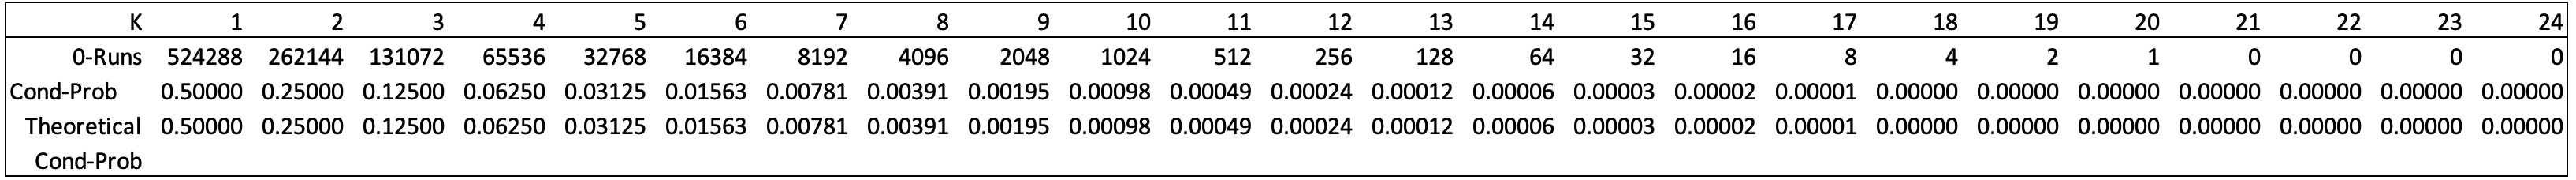
\includegraphics[width=\textwidth]{0_run_table}
		Table 1: Table of 0-run lengths and their probabilities.
	\subsection{A6}
		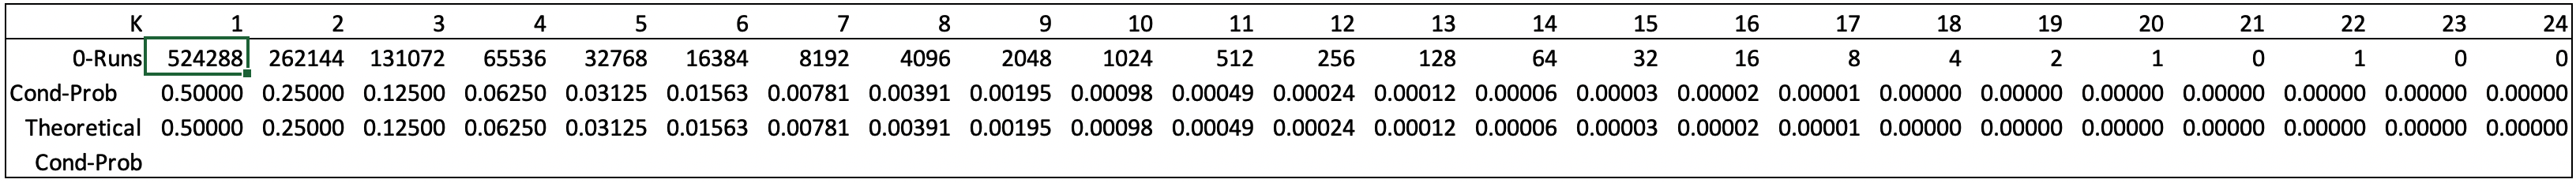
\includegraphics[width=\textwidth]{1_run_table}
		Table 2: Table of 1-run lengths and their probabilities.
\section{Part B}
		\subsection{B2}

		\subsection{B3}

		\subsection{B4}
			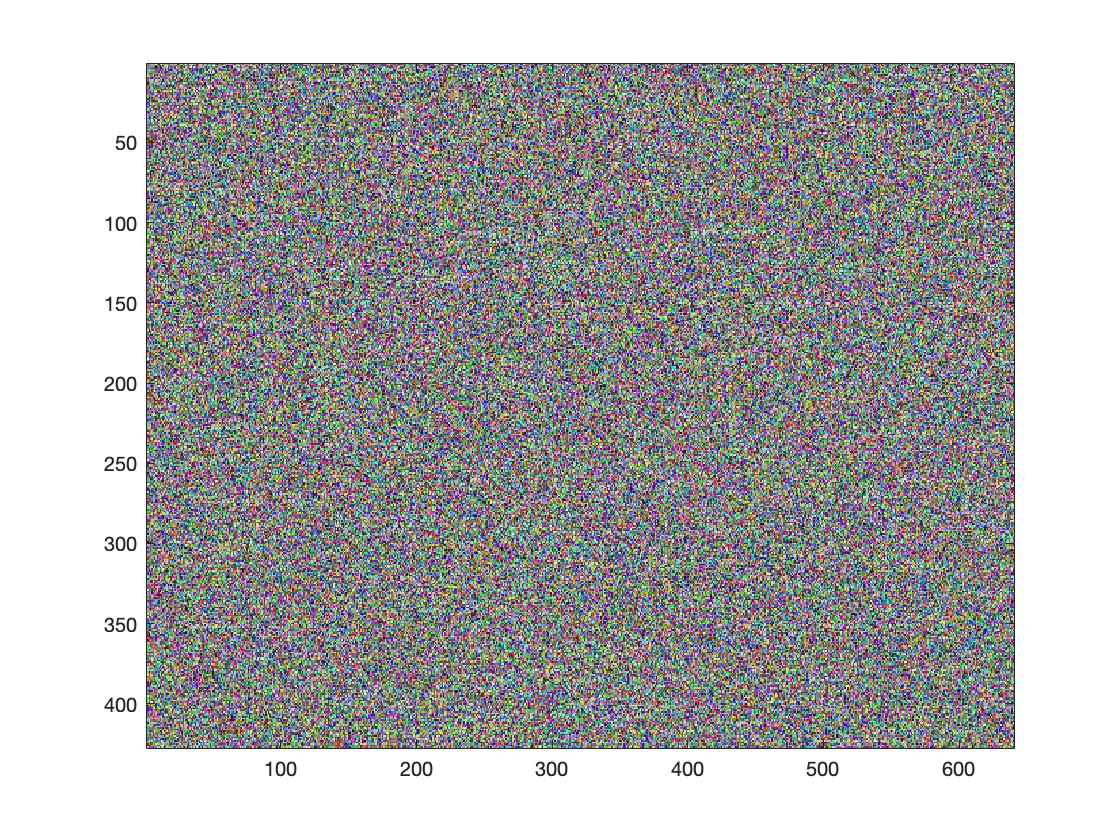
\includegraphics[width=0.45\textwidth]{encrypted_image}
		\subsection{B5}
			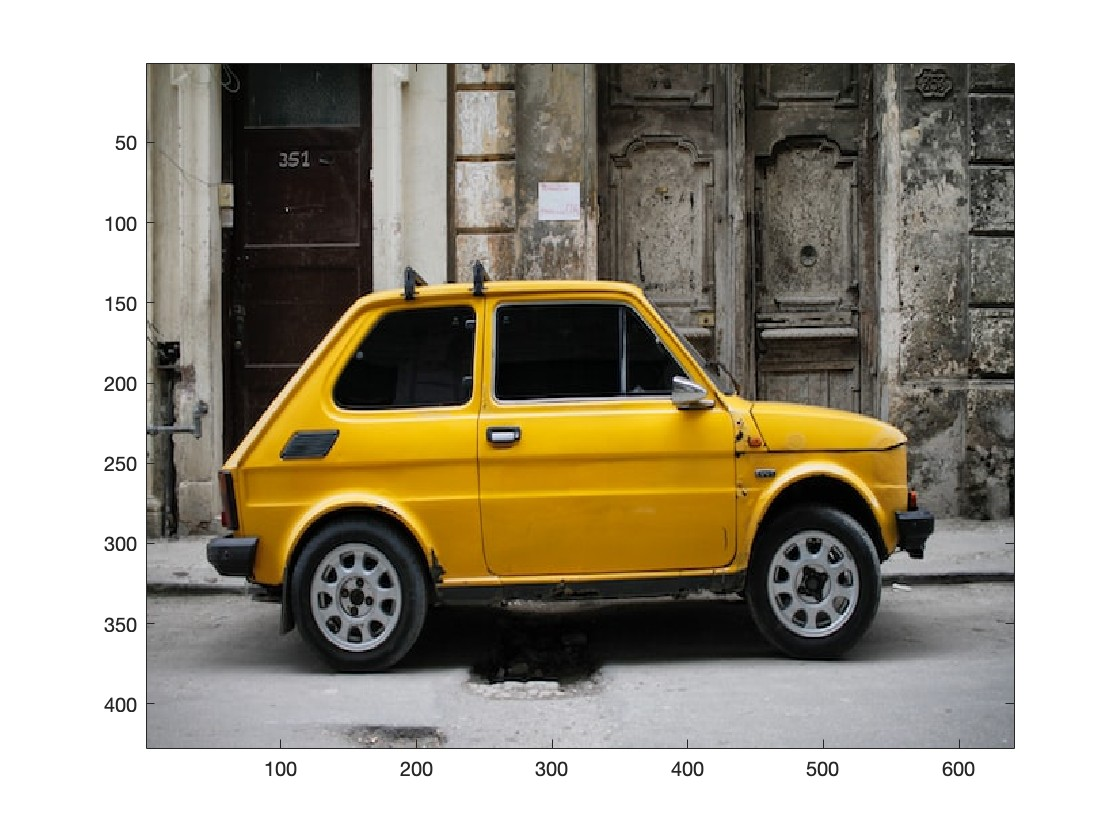
\includegraphics[width=0.45\textwidth]{decrypted_image}

\section{Extra Info}
	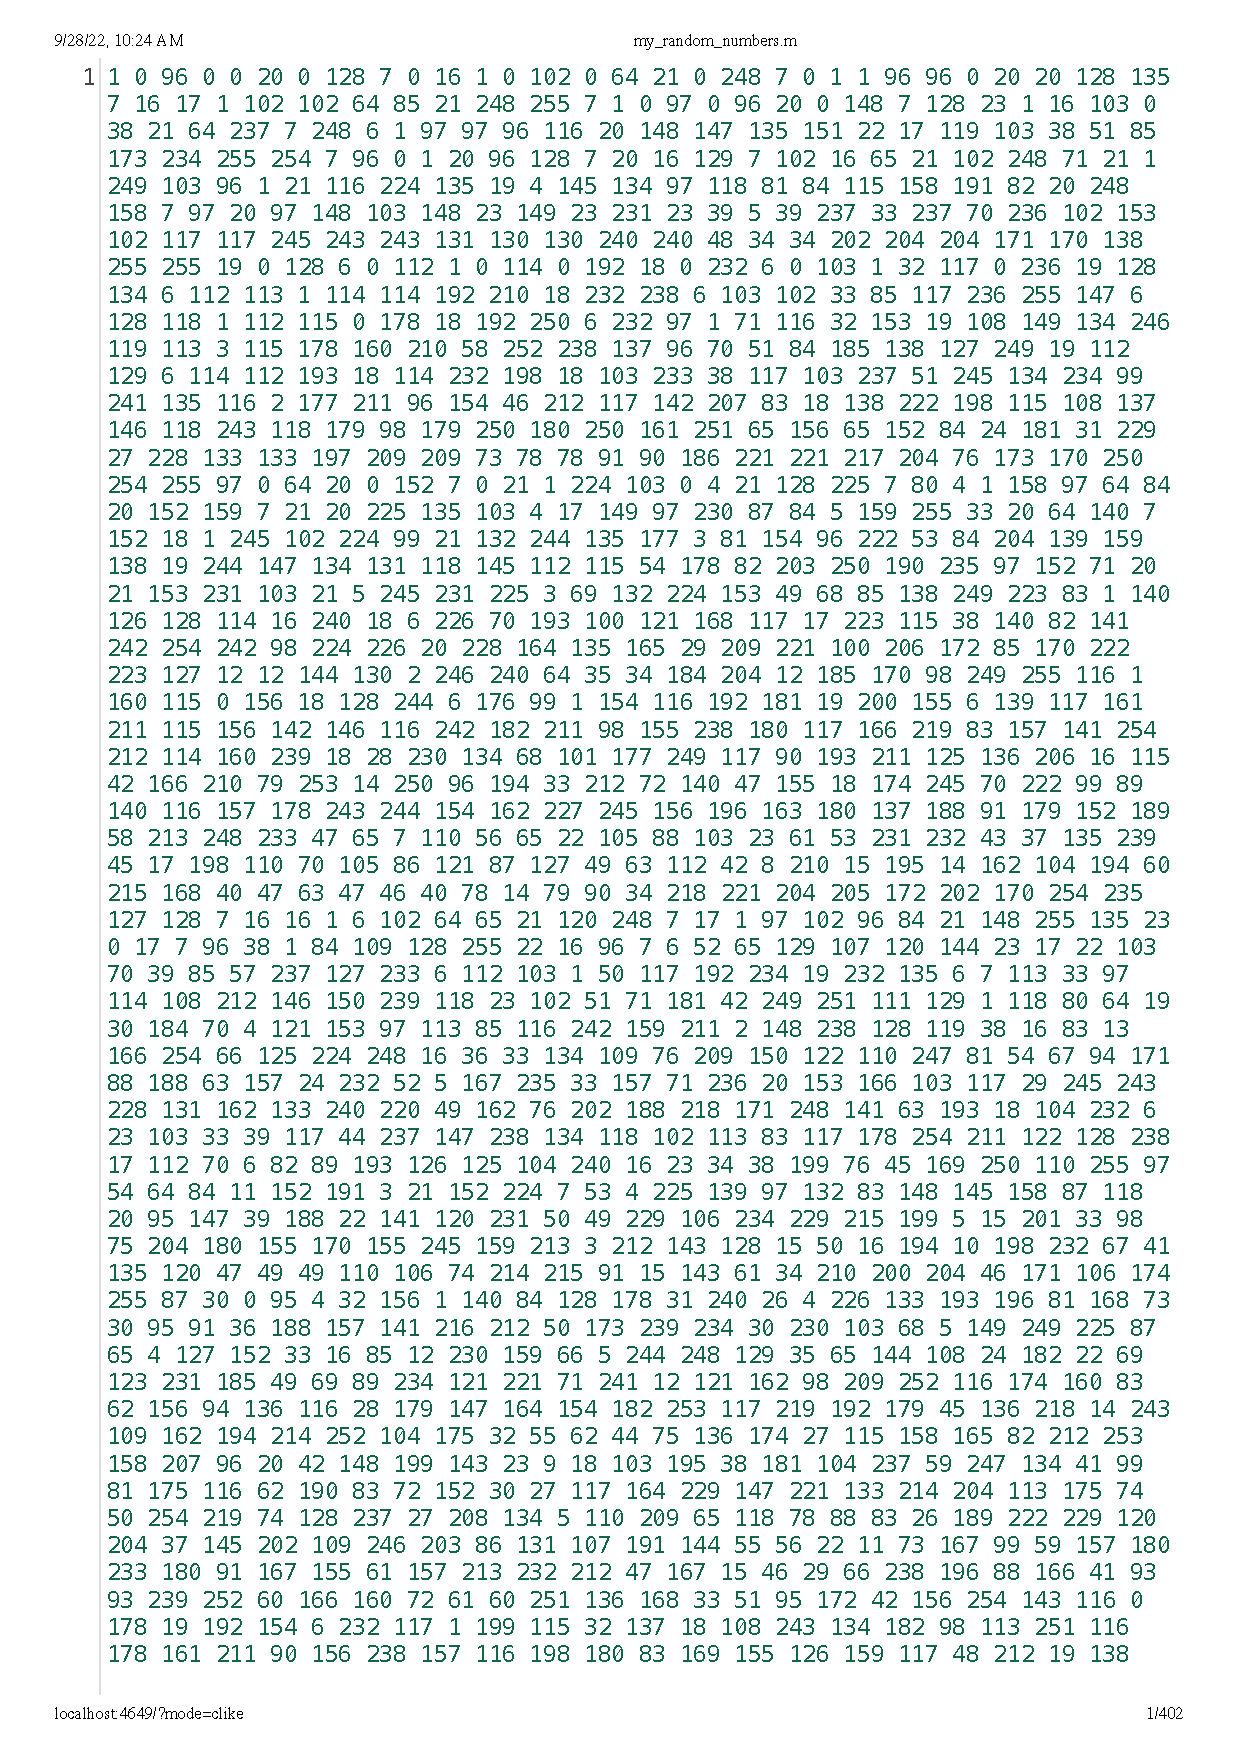
\includepdf[pages=-]{my_random_numbers.pdf}
	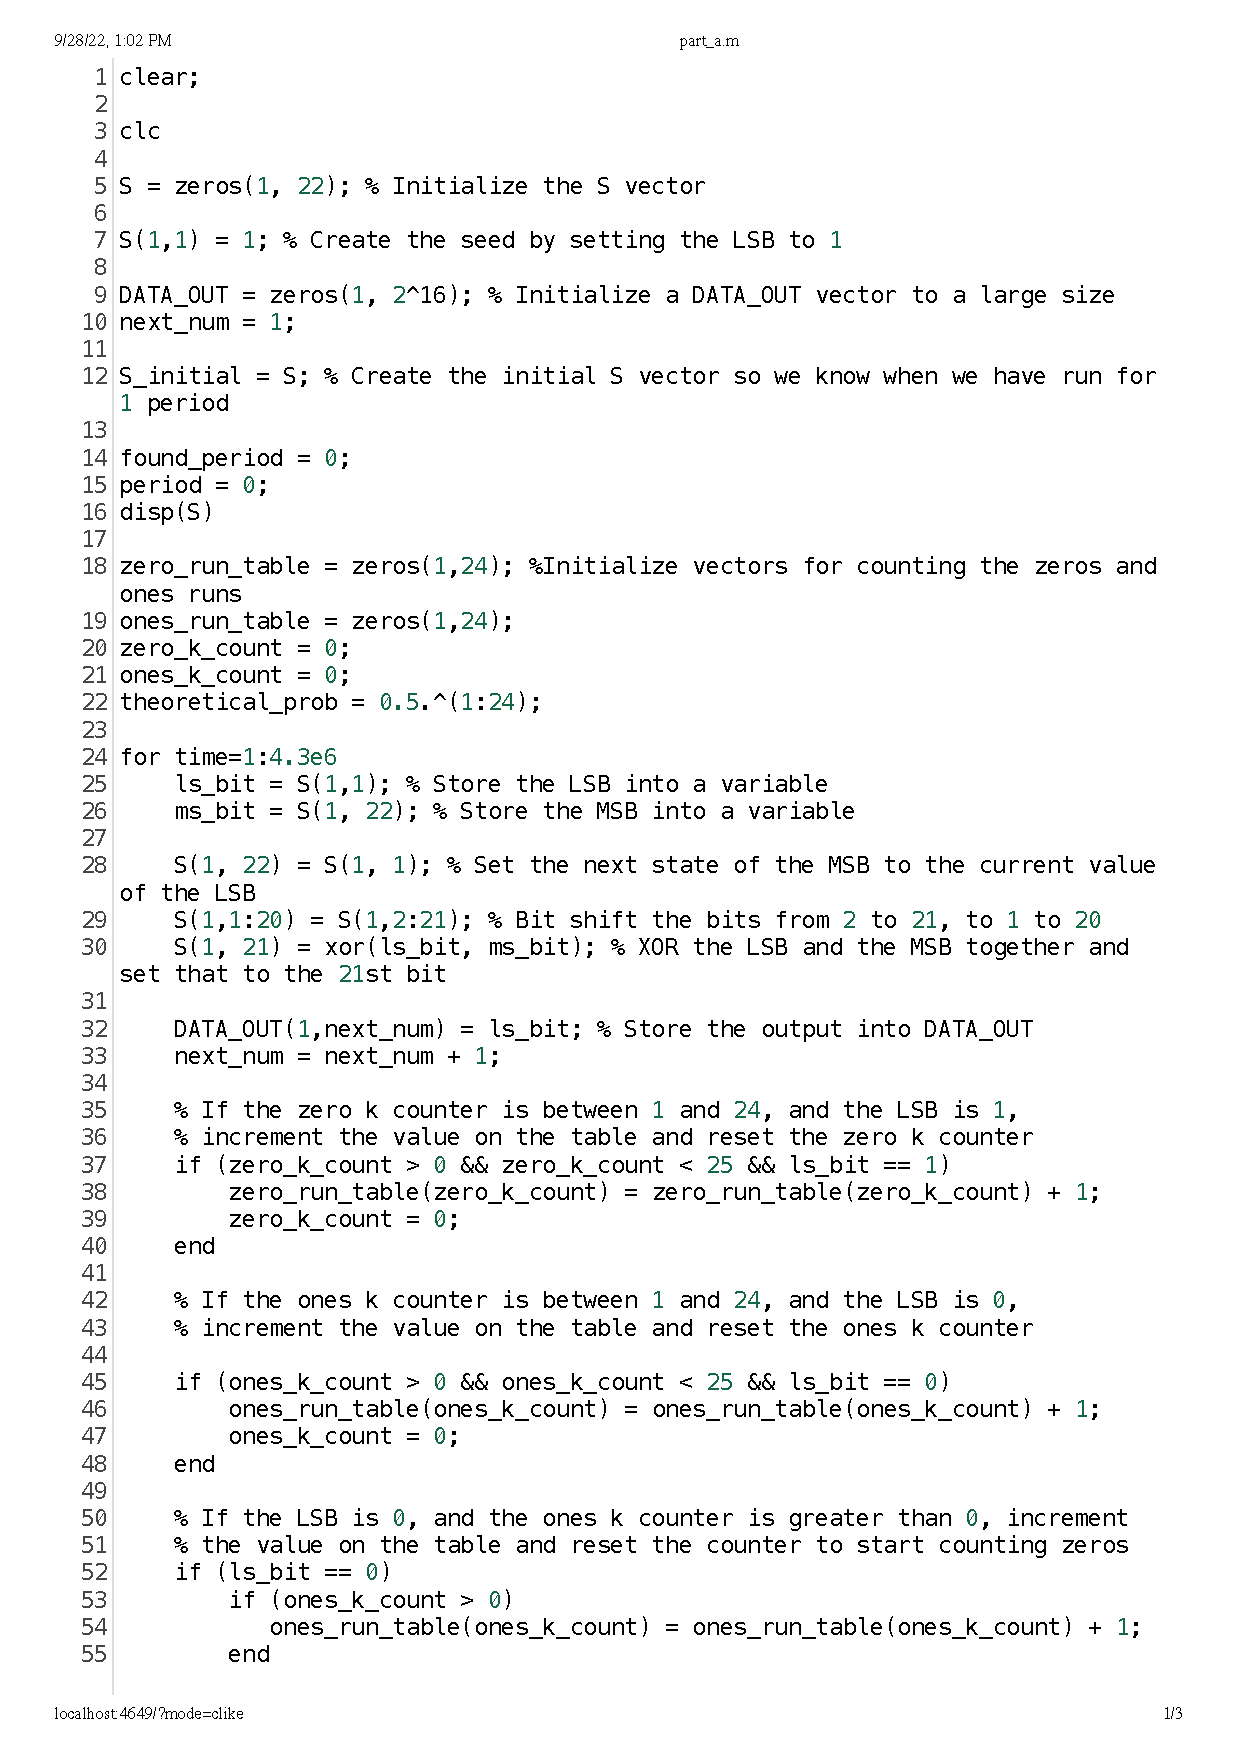
\includepdf[pages=-]{part_a.pdf}
	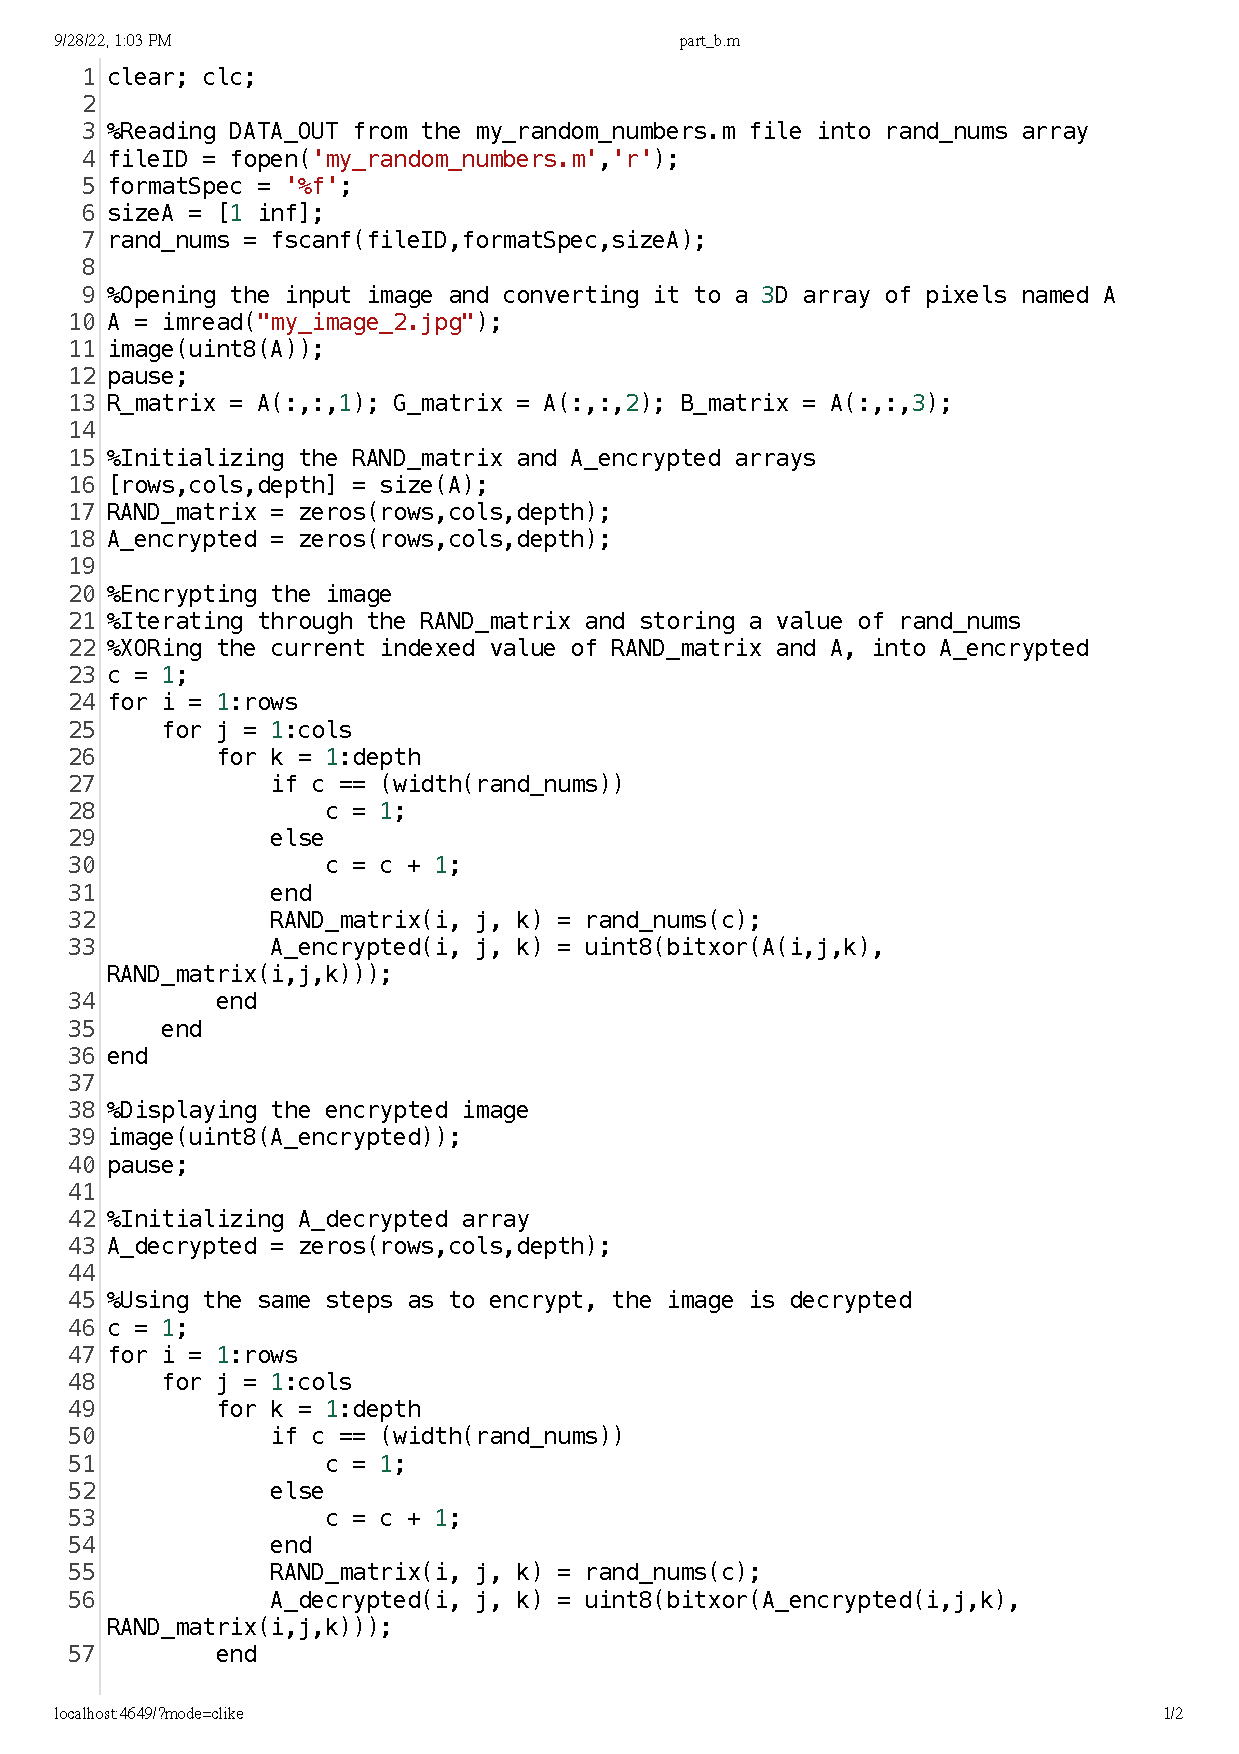
\includepdf[pages=-]{part_b.pdf}
\end{document}          